% Chapter Template

\chapter{Ρομποτική Πλατφόρμα} % Main chapter title


\label{Chapter2} % Change X to a consecutive number; for referencing this chapter elsewhere, use \ref{ChapterX}

%----------------------------------------------------------------------------------------
%	SECTION 1
%----------------------------------------------------------------------------------------

\section{Το Ρομποτικό Όχημα Monstertruck}
\par
Το ρομποτικό όχημα Monstertruck αποτελεί μία ρομποτική πλατφόρμα, που αναπτύχθηκε στα πλαίσια 
της ομάδας P.A.N.D.O.R.A., για συμμετοχή σε διαγωνισμό με θεματολογία την διάσωση θυμάτων σε 
συνθήκες καταστροφής. Η ρομποτική πλατφόρμα είναι κατάλληλη για εφαρμογές χαρτογράφησης, 
εξερεύνησης άγνωστων χώρων και αναζήτησης σημείων ενδιαφέροντος, όπως για παράδειγμα, ανθρώπινα 
θύματα.

\bigskip\par
Για την κατασκευή της ρομποτικής πλατφόρμας, χρησιμοποιήθηκε, σαν βάση, το τηλεκατευθυνόμενο 
όχημα GroundPounder της εταιρείας Redcat Racing. Ανήκει στην κατηγορία φορτηγών οχημάτων 
Monstertruck, με κλίμακα 1:10 και περιλαμβάνει σκελετό από αλουμίνιο, τετρακίνηση, όπως επίσης, 
και ρυθμιζόμενες αναρτήσεις. Επιπλέον, περιλαμβάνει δύο σερβοκινητήρες, για τον ανεξάρτητο 
έλεγχο στρέψης των μπροστινών και πίσω τροχών, προσφέροντας μεγαλύτερη ευελιξία, συγκριτικά με 
τα συμβατικά αυτοκίνητα.\\

\begin{figure}[!h]
	\begin{center}
		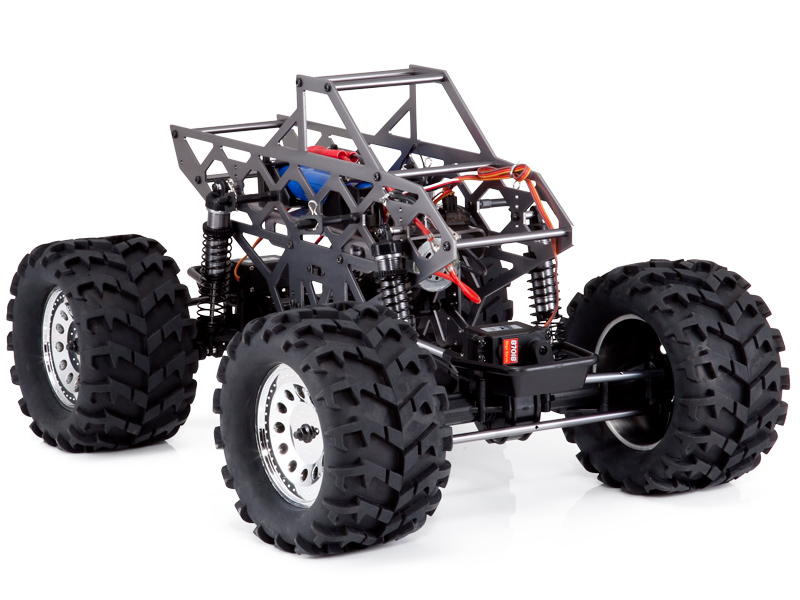
\includegraphics[width=10cm]{Chapters/Chapter2/Figures/groundpounder_chassis.jpg}
		\caption{Το τηλεκατευθυνόμενο φορτηγό όχημα 1:10 GroundPounder}
		\label{fig:groundpounder_chassis}
	\end{center}
\end{figure}

\bigskip\par
Όπως, προαναφέρθηκε, στα πλαίσια της ομάδας P.A.N.D.O.R.A, το παραπάνω τηλεκατευθυνόμενο όχημα 
χρησιμοποιήθηκε σαν βάση, για το τελικό ρομποτικό όχημα Monstertruck. Σχεδιάστηκαν, λοιπόν, και κατασκευάστηκαν, δύο κουτιά, τα οποία τοποθετήθηκαν επάνω στο υπάρχον όχημα, με σκοπό, να περιλάβουν τα ηλεκτρονικά συστήματα του ρομπότ.

\subsection{Κινητήρες}
\subsection{Αισθητήρες}

\section{Κινηματική Ανάλυση}
\subsection{Κινηματικό Ackermann}
\subsection{Κινηματικό 4WS}
\subsection{Προσαρμογή Κινηματικού 4WS στο όχημα Monstertruck}